\documentclass[../thesis]{subfiles}

\begin{document}
	\section{Architecture}
	\label{sec:mic:arch}

	\begin{wrapfigure}{r}{0.3\textwidth}
		\centering
		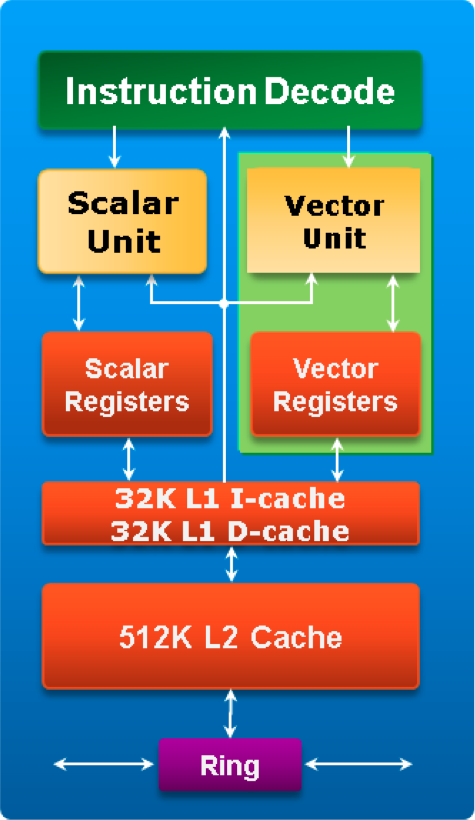
\includegraphics[width=0.25\textwidth]{assets/images/mic/arch/core.png}
		\captionsetup{font=small}
		\caption{\intel MIC Architecture core diagram.}
		\label{fig:mic:core}
	\end{wrapfigure}

	\tdg{\# of cores, frequency and cache}
	The \intel\xeon Phi Coprocessor contains up to 61 fully functional in-order \intel\mic Architecture cores running at 1GHz (up to 1.3GHz), each containing 64KB of L1 cache (evenly split for data and instructions) and 512KB of L2 cache.

	\tdg{Memory}
	The device can support 8 memory controllers with two \gddr5 channels each. These support a total of 5.5 GT/s, corresponding to a theoretical aggregate bandwidth of 352 GB/s. So far, the maximum memory size available is 16GB\footnote{\intel\xeonphi Coprocessor 7120X \cite{intel:datasheet:xeonphi}}.

	\begin{figure}[!t]
		\centering
		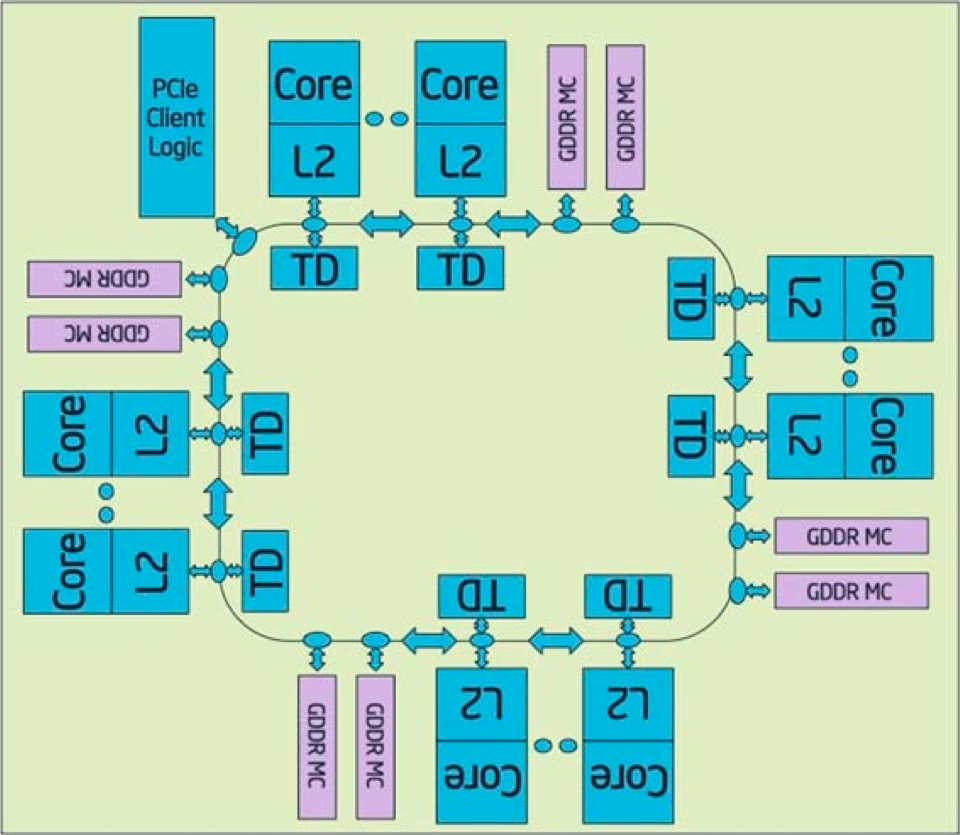
\includegraphics[height=0.3\textheight]{assets/images/mic/arch/microarch.png}
		\caption{Knights Corner Microarchitecture}
	\end{figure}

	\tdg{Ring, LL cache and coherency}
	A high performance on-die bidirectional ring connects the L2 caches, the memory controllers and the \pcie interface logic. The connected L2 caches allow for requests to be fulfilled from other cores' L2 caches faster than it would be from memory, thus implementing a last-level cache with over 30MB. Cache coherency is preserved across the entire coprocessor through a distributed tag directory using a reversible one-to-one hashing function.

	\tdg{ISA}
	\intel\mic Architecture is based on the x86 \isa, extended with 64-bit addressing and 512-bit wide \simd vector instructions and registers. Yet, it does not support other \simd\isas (\mmx, \intel\sse and \intel\avx).

	\tdg{Architecture of the cores}
	Each coprocessor core supports up to 4 hardware threads and can execute 2 instructions per clock cycle, one on the U-pipe and one on the V-pipe (not all instructions can be executed in the latter). Each hardware thread has a ``ready-to-run'' buffer comprising two instruction bundles, each bundle representing two instructions that can be executed simultaneously.

	\tdg{Vector capabilities}
	The \vpu contains 32 vector registers, each 512-bit wide. It includes the \emu and is able to execute up to 16 integer or single-precision floating-point operations per cycle (half for double-precision). Additionally, each operation can be a floating-point multiply-add, thus doubling the number of operations in each cycle. Fully utilizing the \vpu is critical to achieve high performance with the coprocessor.

\end{document}
